\documentclass{article}

\renewcommand{\rmdefault}{ptm}
\renewcommand{\sfdefault}{phv}
\usepackage[top=30truemm,bottom=30truemm,left=25truemm,right=25truemm]{geometry}
\widowpenalty=10000
\clubpenalty=10000
\flushbottom
\sloppy
\usepackage{natbib}

\usepackage[utf8]{inputenc} % allow utf-8 input
\usepackage[T1]{fontenc}    % use 8-bit T1 fonts
\usepackage{hyperref}       % hyperlinks
\usepackage{url}            % simple URL typesetting
\usepackage{booktabs}       % professional-quality tables
\usepackage{amsfonts}       % blackboard math symbols
\usepackage{nicefrac}       % compact symbols for 1/2, etc.
\usepackage{microtype}      % microtypography
\usepackage{placeins}

\usepackage{bm}
\usepackage{xspace}
\RequirePackage{algorithm}
\RequirePackage{algorithmic}
  \RequirePackage{natbib}
\usepackage{wrapfig}
\usepackage{subcaption} 
\usepackage{multirow}
\usepackage{adjustbox}
\usepackage{amsmath}
\usepackage{graphicx}

\usepackage{todonotes}
\usepackage{enumitem}

%\usepackage{ragged2e}
\DeclareMathOperator*{\argmax}{arg\,max}
\usepackage{array}
\newcolumntype{L}{>{\centering\arraybackslash}m{3cm}}



\title{Bayesian Learning for LambdaZero}

\date{}
\begin{document}
\maketitle

\section{Problem Formulation}

\todo{Got the timings for this values for this section from various emails/messages -- need to check that they are actually correct!}

We want to search for molecules, $m$, over chemical space, $m \in \mathcal{X}$, using LambdaZero.
In particular, we want to find a small organic molecule that binds to the COVID-19 protease. 
This binding ability can be experimentally measured (using a bilogical assay), $y_a: \mathcal{X} \to \mathbb{R}$, 
where this process is subject to some noise $y_a(\cdot) = f_a(\cdot) + \epsilon_a(\cdot)$.
There is a budget for testing ~50 molecules this way at a time.
The overall goal is to find $m^\ast = \argmax_{m \in \mathcal{X}} f_a(m)$ , subject to $c_i(m) \geq C_i$ for $i=1,\ldots, n$,
where the $c_i(\cdot)$ represent constraints such as toxicity, ease of synthesis etc.

\paragraph{Computational Approximations to Binding Affinity} To help us do this we also have access to the following computational functions to use as oracles
(all deterministic),$f_{\cdot}: \mathcal{X} \to \mathbb{R}$,  which predict the binding ability:
\begin{description}[font=\normalfont\sffamily]
  \item[Cheap Docking ($f_D$):] This takes ~15 secs per molecule. This is computed using \href{http://dock.compbio.ucsf.edu/DOCK_6/index.htm}{Dock6} or
    \href{https://ccsb.scripps.edu/autodock/}{AutoDock},
    which takes as input the ligand's graph (ie the graph of the small organic molecule) and the 3D structire of the protein. 
    It outputs the interaction energy and geometric coordinates of the top scoring poses 
    (see \href{http://dock.compbio.ucsf.edu/DOCK_6/tutorials/ligand_sampling_dock/ligand_sampling_dock.html}{here} for further details).
  \item[Expensive Docking ($f_{ED}$):] This takes ~8 min per molecule. 
    Uses the same software as the cheap docking with different parameters. 
  \item[Free Energy Perturbation ($f_{FEP}$):] This takes approximate 1 day per molecule on specialized GPU hardware.
    This could be done using eg the \href{https://www.schrodinger.com/fep}{FEP+ software} \citep{Wang2019-zm, Ciordia2016-xn}.
    See \citep{Shirts2010-mx} for an overview of this method.
\end{description}

These different computational functions come with different costs (in terms of runtime) and expected accuracies. 
Also for some of them we are able to send a batch of molecules to query at once.
We summarize the costs of the different techniques in the table below (Table \ref{table:oracles_and_costs}) along with the number of evaluations we expect to obrain.

\begin{table}[H]

  \begin{tabular}{lLLLL}
  \hline
    Method            & Variance of error distribution & Runtime per molecule       & Number of batches that can be queried & Size of batch \\
\hline
Cheap Docking     & 2.5-2.7                        & $\sim$15 secs              & 200E6                                    & 1             \\
Expensive Docking & 2.5-2.7                        & $\sim$8 mins               & 1E6                                      & 1             \\
FEP               & 0.7-1.5                        & $\sim$1 Day (GPU hardware) & 50                                       & 256           \\
Lab Experiment    & 0.3-0.5                        & 1 week+ (in a lab)         & 5                                     & 15           \\
\hline
\end{tabular}

\caption{Table showing (i) the variance of the error distribution of each method (this is when measuring negative binding energy in kCal/mol
which, when measured over all molecules, we expect to be in the range -16 to 0.), (ii) the runtime to compute the operation over one molecule,
(iii) the number of batches we can afford to send to each oracle (iv) the size of each batch which can get sent to each oracle.
}
\label{table:oracles_and_costs}
\end{table}


We also can train surrogate models (eg using a graph neural network, or fully connected neural network on molecular fingerprints)
to predict the outputs of these computations in a much faster time (around 5ms). 
When using we will denote these wrt to the underlying geometric/statistical mechanical computations they are acting as a proxy for,
eg $\hat{f}_{ED}^\theta$.




\paragraph{Initial Molecular Dataset} Before LambdaZero is operational and generating novel molecules, and in order to gather data to train its reward function/extract a vocabulary of molecular building blocks,
we also can get access to a a large set of initial obtainable molecules, $\mathcal{M} = \{m_1, m_2, \ldots, m_{|\mathcal{M}|}\}$,
with $\mathcal{M} \subset \mathcal{X}$.
In particular, we are interested in using the ZINC database \citep{Irwin2012-gf} for this purpose,
where $|\mathcal{M}_{\textrm{ZINC}}| \approx 200 \textrm{million}$. 
The idea would be to run the cheap docking described above on all of these molecules.
Note that this would be done in parallel on eg AWS (taking about 7 days) and although the calculation for each molecule is relatively fast,
over the whole database
this would amount to a considerable computation (15secs $\times$ 200 million $\approx$ 95 years if computed serially!).

\subsection{Where Bayesian Learning might help?}

On the calls/emails we have discussed several places where Bayesian learning may improve the speed/cost of solving the problem:

\subsubsection{Gathering initial data before LambdaZero takes over}
Before LambdaZero is trained there is an opportunity to collect data from both the in silico models and in vitro experiments 
discussed previously.
Two different possible aims of this work have been discussed:

\vspace{0.1cm}
\noindent
\textbf{Possible Task 1.} As a \emph{Bayesian optimization problem} (BO) \citep{pmlr-v89-song19b, pmlr-v70-hernandez-lobato17a} to find the best molecule from $\mathcal{M}_{\textrm{ZINC}}$.
Can think of this as encompassing BO into a virtual screening approach.
This would try to aim straight away to find a suitable thereaputic molecule from a set of molecules that are already acquirable
and so more quickly physically testable. 
It would aim to find the best known molecule which then LambdaZero would have to try to improve upon by exploring novel molecules.

\vspace{0.1cm}
\noindent
\textbf{Possible Task 2.} As an \emph{active learning} \citep{pinsler2019bayesian, kirsch2019batchbald} problem where the aim is to learn a surrogate model
$\hat{f}^\theta_a$, which works well over all of $\mathcal{X}$ and is used as part of a fast-to-query reward function in LambdaZero.
This may differ from the first problem by expending computation on areas of molecular space that are known to have poor bind affinities 
so that it can still give LambdaZero accurate rewards there.


\vspace{1cm}
Both of these tasks share common problems, namely:
\begin{itemize} 
  \item how best to query between different oracles of different costs and fidelities,
  \item how to choose a batch of points to send to an oracle at once,
  \item how to optimize an acquisition function over hundreds of millions of discrete candidates,
  \item how best to design the surrogate models with well-callibrated uncertainties, whilst quick to train and query,
\end{itemize}


\subsubsection{Encouraging diversity and exploration in LambdaZero}
We have also discussed whether the BO described above should continue when LambdaZero is able to generate novel molecules. 
Again this could be done in multiple ways:

\vspace{0.1cm}
\noindent
\textbf{Possible Task 3.} At each iteration step when choosing to send off a molecule to one of the more expensive oracles BO is used to pick
between the molecules LambdaZero has generated and those belonging to $\mathcal{M}_{\textrm{ZINC}}$.

\vspace{0.1cm}
\noindent
\textbf{Possible Task 4.} Use BO to define the acquisition function that LambdaZero then needs to optimize when finding molecules. 
That is instead of optimizing for docking (or a surrogate model thereof) LambdaZero's reward is an acquisition function 
computed using the principles of BO.
This would encourage diverse and novel outputs from LambdaZero, as the acquisition function would be controlling
the exploration/exploitation trade-off.
However, the reward function for LambdaZero would become more complicated.
The state in MCTS (Monte Carlo Tree Search) would also have to encompass a notion of the data seen so far
(perhaps agglomerated eg via \citep{NIPS2017_6931, skianis2019rep}
as well as the current
junction tree scaffold of the working molecule, as the reward from the acquisition function would depend on both.

\subsection{Summary: Currently focusing on task 1}

I think at the moment the focus is on task 1, as it would be more immediately useful.


\section{Overview of currently proposed approach}
\label{sect:approach}

In this section we describe the current proposed approach.
Summaries of some design choices is given in Section \ref{sect:design_choices}. 

The overall process is shown in Figure \ref{fig:process}. 
We propose on using two machine learning models: ML Model A and ML Model B.
ML Model A is used to try to correct for any mistakes in cheap docking (after seeing some expensive docking results) and so
collect promising molecules that might not be selected based on cheap docking alone.
ML Model B is a ML model with uncertainties (eg  Bayesian regression on MPNN embeddings or a Gaussian process).
This acts as a gatekeeper for selecting which molecules get sent for expensive FEP simulations.

\begin{figure}[t]
\centering
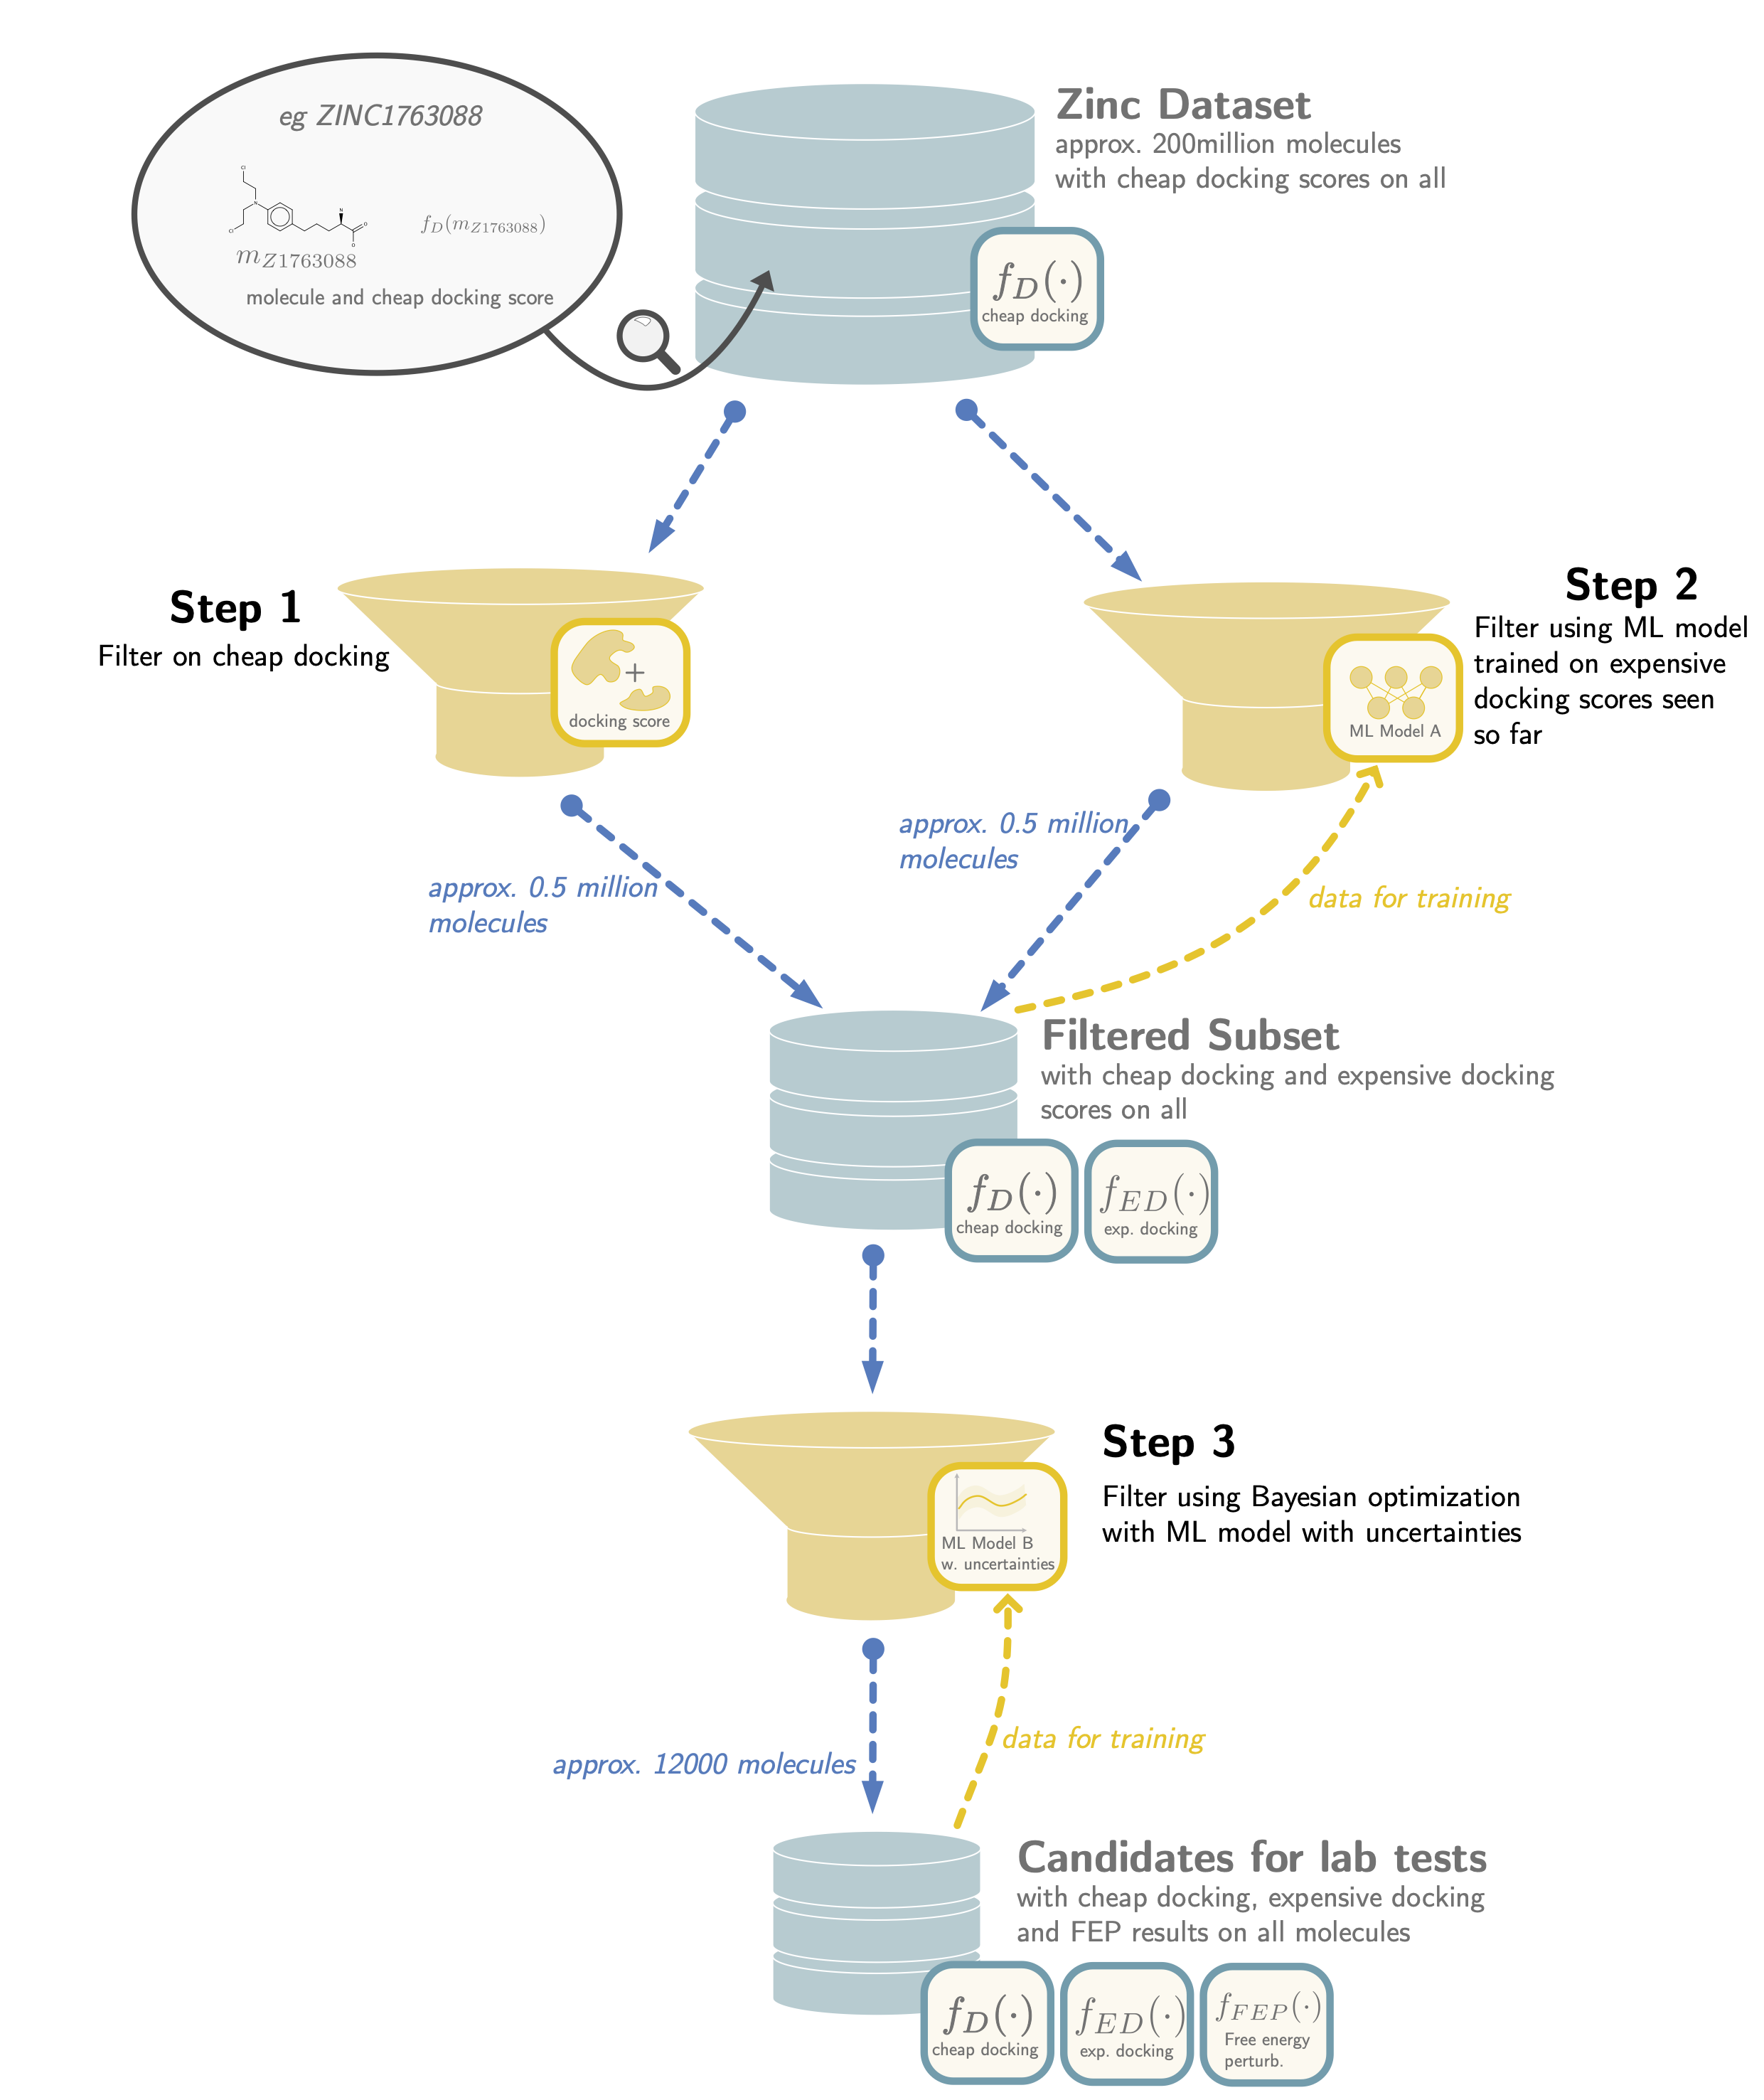
\includegraphics[width=0.9\textwidth]{imgs/process.pdf}
\caption{Overall process of how we propose on selecting which molecules get sent to the more expensive oracles.}
\label{fig:process}
\end{figure}

These ML models would take in as input the scores from the less expensive oracles (which have already been calculated) as well as a
fingerprint representation. Initially for testing this could be a pre-specified fingerprint (eg Morgan Fingerprints) however it is hoped
that this will also be learnt eg using a MPNN (Message Passing Neural Networks) or other network which takes the geometry of the molecule into
account and is trained to predict cheap/expensive docking and molecule orientations recieved from the previous molecules.
A summary of this network is Figure \ref{fig:network}.

\begin{figure}[h]
\centering
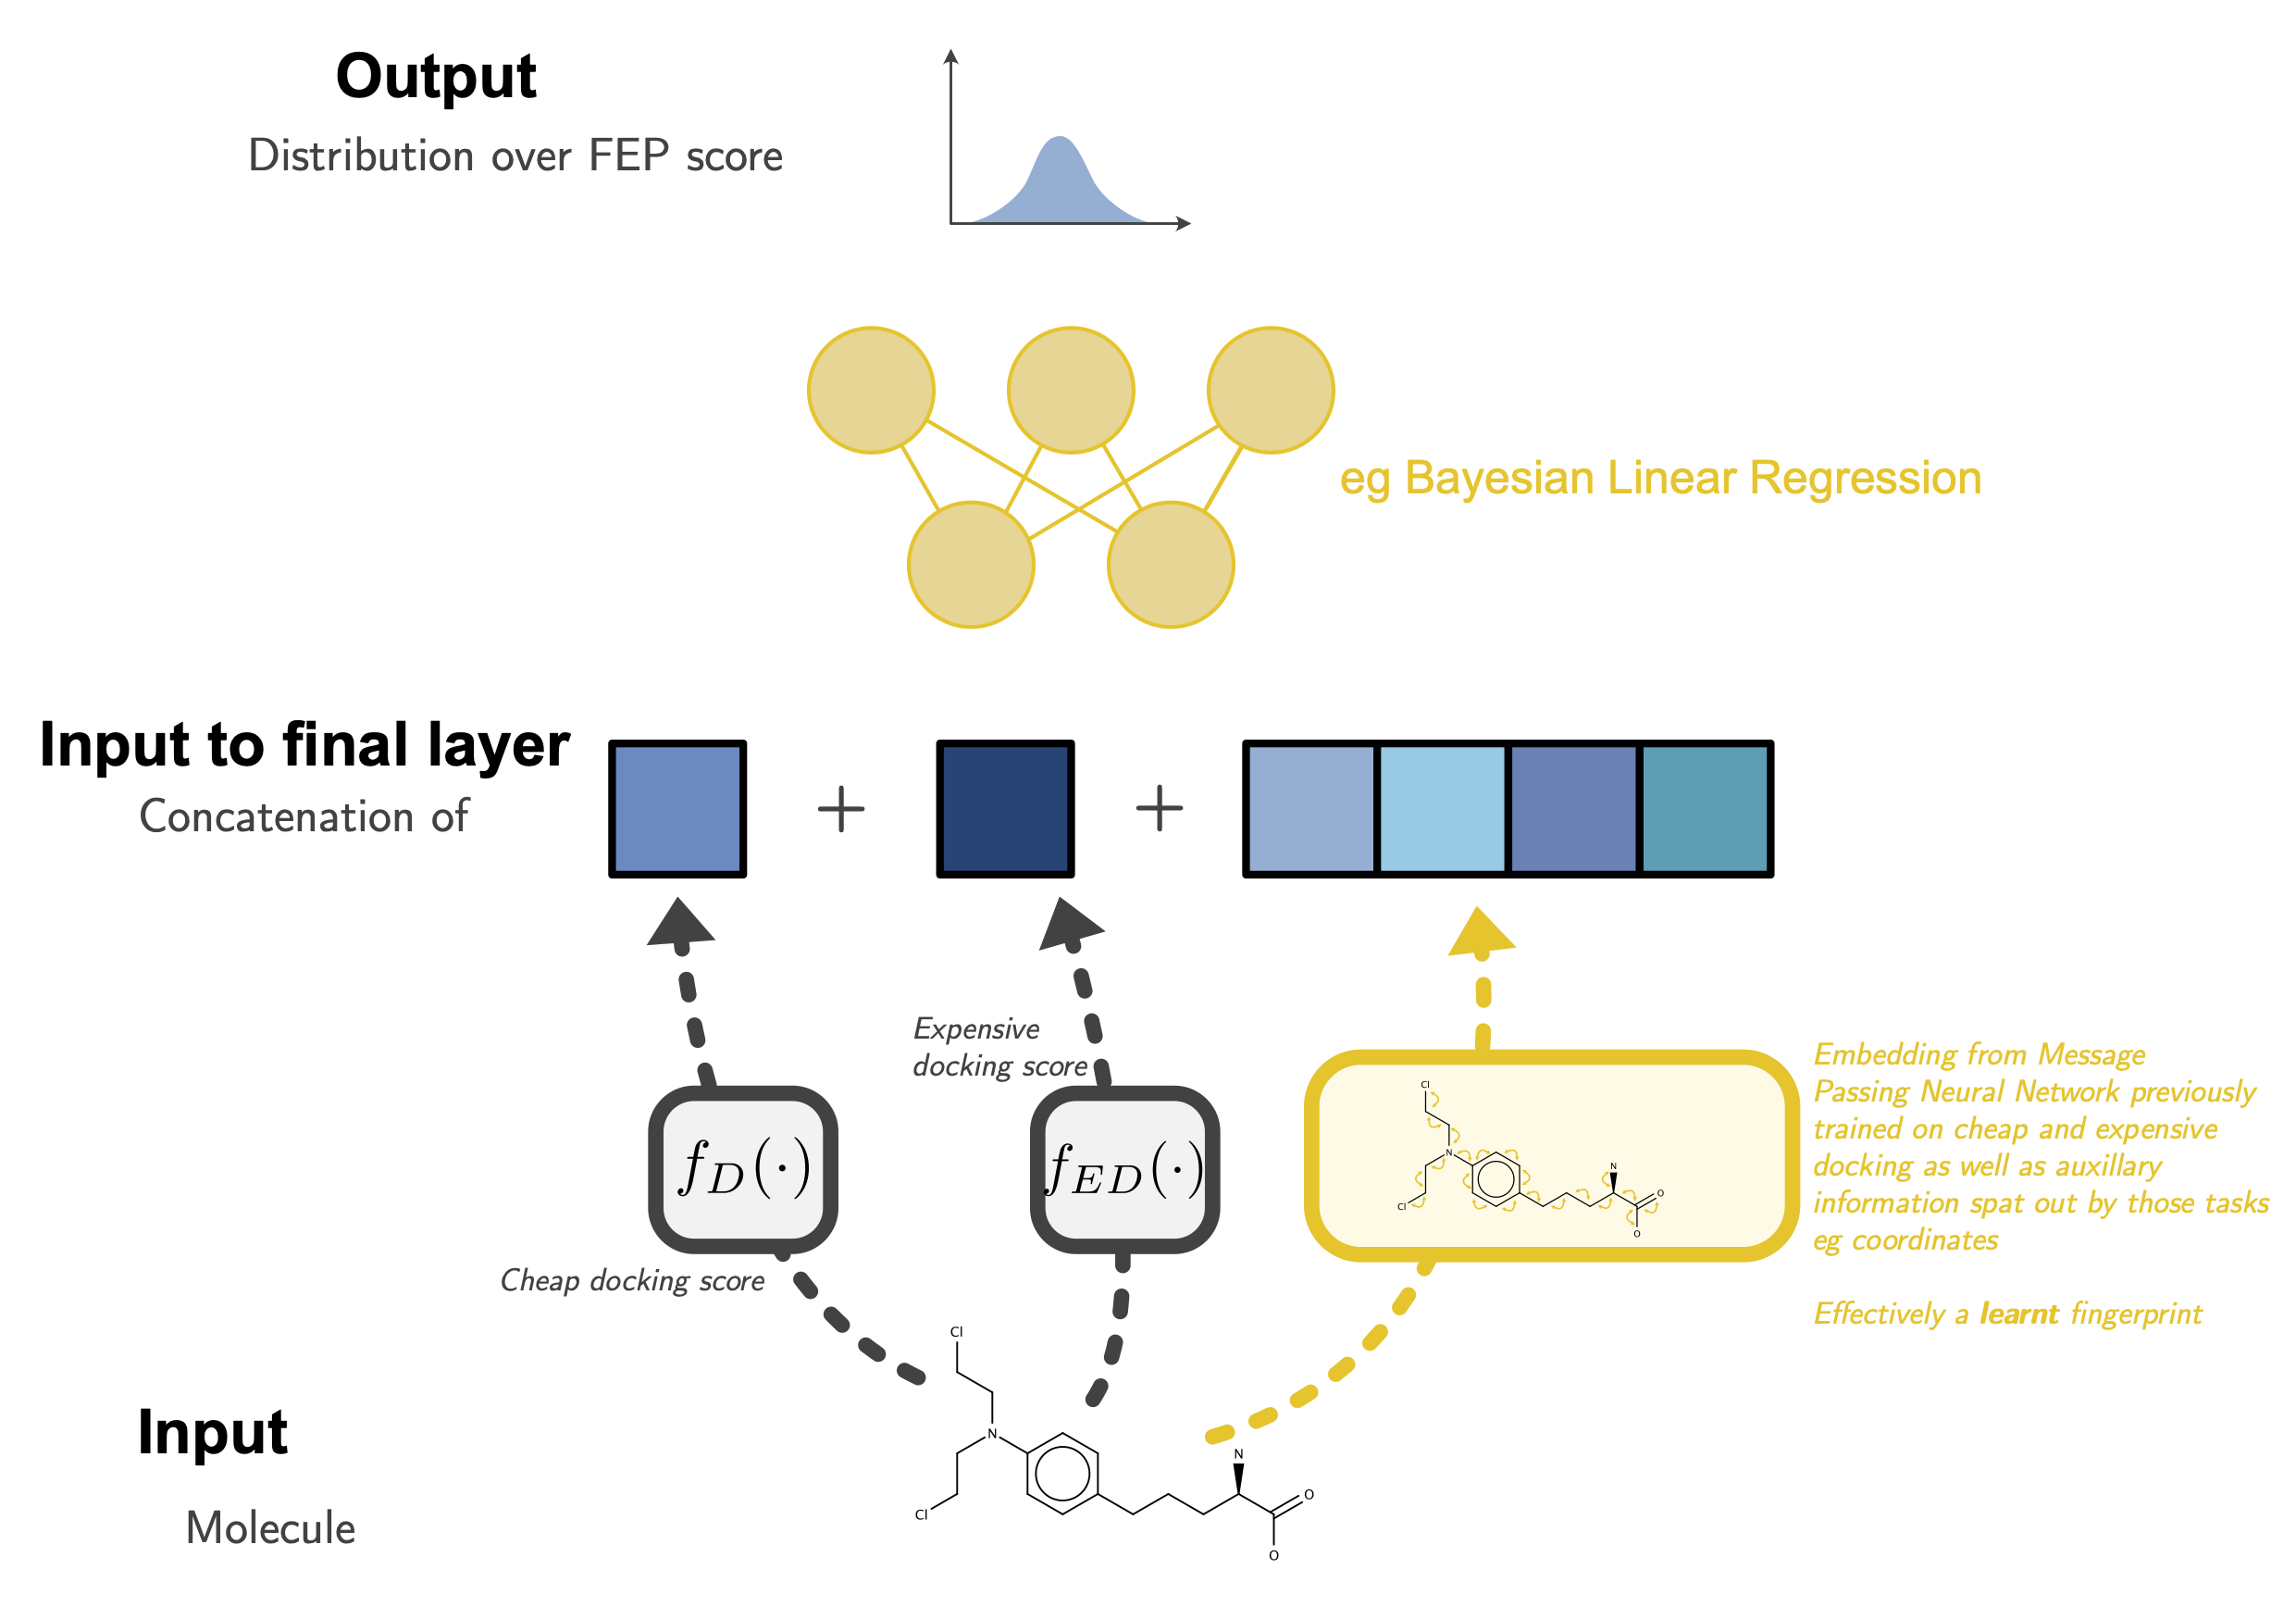
\includegraphics[width=0.9\textwidth]{imgs/networks.pdf}
\caption{The overall architecture of how ML Model B might look}
\label{fig:network}
\end{figure}


\FloatBarrier



\section{Discussions about design choices}
\label{sect:design_choices}


\subsection{Optimizing an acquisition function over a large candidate set}

Running Bayesian optimization over 200 million molecule candidates would take a considerable amount of time/compute
(eg 5ms $\times$ 200million $\approx$ 12 days serially!),
whereas the expensive docking calculation costs only 8 minutes and FEP 1 day.
In this section we discuss various approaches to overcome this problem.
These can be grouped into two categories: the first involves filtering down the dataset using the cheaper simulations
so that any BO  acquisition function is evaluated over the whole of a much smaller subset, whereas the second involves using auxillary ML models to enable
the fast search over which molecules to evaluate the acquisition function on.
We discuss both in further detail below.

\subsubsection{Filtering out the data and running BO only for the most expensive simulations on a reduced dataset}
\label{sect:filter}
\textbf{Pros:} Simple and likely to work; \textbf{Cons:} might miss a promising molecule.


This approach aggressively filters down the dataset size (using the values obtained from the cheap docking),
and only evaluates the acquisition function on the reduced set size. 
The approach is a traditional virtual screening approach with BO only used for the most expensive simulations
at the end.

\begin{itemize}
\item From 200 million it could be that the cheap docking rules out a large proportion
and could be used for filtering without any ML model.
\item Then approximatley 1 million could be evaluated using the expensive docking. 
\item For FEP (a day long operation) we could then start using BO, and evaluate an acquisition function on all 1 million
  ($5ms \times 1E6 \approx 1hr 20mins$) to pick a 12k subset which get sent to the FEP simulation. \todo{check these figures!}
\item Periodically after improving our surrogate models we could go back and revaluate them on the 200 million full dataset
to catch any molecules potentially incorrectly filtered out by the cheap docking.
\end{itemize}

\noindent
Practically the whole workflow might look something like this:
\paragraph{Beforehand} Evaluate cheap docking, $f_D$, over the whole 200 million of $\mathcal{M}_{\textrm{ZINC}}$. 
There are ?? processors for this and it takes 15 secs per molecule, with the results expected in ??.
\paragraph{Step 1} Using the half million molecules with the best cheap docking score, $\mathcal{M}_{D\ast,1E6}$, run
expensive docking, $f_{ED}$, on these molecules. There are ?? processors for this and it takes 8 mins per molecule, so the
results are expected in roughly ?? days after step 1 is complete.
\paragraph{Step 2a} 
Simultaneously with step 2a train a GNN, $\hat{f}_D^\theta: m \to \mathbb{R}$,
to extract vector embeddings from molecules (from eg its penultimate layer) useful for downstream tasks.
This network could be trained to predict $f_ED$. 
\paragraph{Step 2b} Create features for each molecule in $\mathcal{M}_{D\ast,1E6}$ through the concatenation
of the embeddings created in step 2b, the cheap docking score, and the expensive docking score ie
$\bm{x}_i = f_D(m_i) \| f_{ED}(m_i) \| \hat{f}_{D, \textrm{penultimate layer}}^\theta(m_i) $.
Over 1 GPU machine this might take a couple of hours to compute.
\paragraph{Step 2c} Using this model also select another half milltion molecules for expensive docking evaluation.
\paragraph{Step 3} Run eg Batch Thompson Sampling \citep{pmlr-v70-hernandez-lobato17a} for working out which
$m_i \in \mathcal{M}_{D\ast,1e6}$ get the FEP evaluated on, $f_{FEP}$. 
The BO would use involve training a Bayesian NN or GP to predict $f_{FEP}$, using $\bm{x}_i$ in as features.





\subsubsection{Cluster the data and only evaluate the molecules in the most promising cluster}

Run clustering on the 200 million dataset, eg by using streaming k-means, to break the data down into smaller
clusters (these cluster could be further broken down into sub-clusters to form a tree structure).
When optimizing the acquisition function first evaluate the function on the mean of each cluster,
and only evaluate further the members of the most promising cluster.



\subsubsection{Two-level Bayesian optimization}

\textbf{Cons:} Untested and so could come across problems when trying this in practice.

Optimizing the acquisition function could be viewed as a Bayesian optimization problem itself.
We could solve this search over a fixed 200 million discrete space by using the VAE approach from \citet{gomez2018automatic}
but restricting the molecules output by the decoder to elements of this discrete set. 
Then optimization over the 200 million could be done with far less evaluations moving about the continuous latent space
of the VAE using an outer loop of BO.

To restrict the decoder to output only valid and already-defined molecules, we could use a CVAE (character VAE).
Before training this we would build a \href{https://en.wikipedia.org/wiki/Trie}{trie} from the 200 million SMILES strings in
$\mathcal{M}_{\textrm{ZINC}}$, to collect all the valid SMILES string prefixes.
This trie datasructure be used inside the decoder to provide masking when picking the next character at each step.

Alternatively, we could train a decoder to predict a fingerprint representation
(either eg pre-defined fingerprint such as \citet{Rogers2010-tv} or one output by a GNN \citep{duvenaud2015convolutional})
which we then match to its nearest neighbour in $\mathcal{M}_{\textrm{ZINC}}$, which we are selecting from.

In order to regularize the VAE to have a well-structured latent space we could simultaneously train a regressor from the latent 
molecule embedding to the value of the cheap docking binding affinity when training the ordinary ELBO.

When optimizing the acquision function for selecting which molecule to send to the FEP oracle we would not evaluate it
over all 200 million members of $\mathcal{M}_{\textrm{ZINC}}$. 
Instead the acquisition function would be evaluated over a much smaller subset of molecules selected by running a second loop
of BO in the VAE's latent space.

\subsubsection{Summary: currently focusing on the filtering approach (\S\ref{sect:filter})}
As simpler and faster to implement currently focussing on filtering out using the cheaper oracles and only using BO before FEP.





\bibliography{refs}
\bibliographystyle{plainnat}


\end{document}

